\cotefile{78}
\scanpage{75}
\noindent\begin{tabular}{||p{.9\linewidth}}\unsure{Réalisation|Réalisations} géométriques des polyèdres \deleted{\unsure{infinis|affines}} combinatoires
en coordonnées affines universelles.\end{tabular}

\uline{1}. Programme de travail.

\deleted{\unsure{1.}} \uline{1}. Soit $\Pi$ polyèdre combinatoire donné, on se
propose d'étudier ses réalisations géométriques \inserted{régulières}
dans des \deleted{\unsure{espaces}} \inserted{plans} affines variables $E$. Notons
que si deux telles réalisations sont $\Pi$-isom, il y
a un $\Pi$-isom \uline{unique} entre elles, par
définition. Donc dans tte classe d'isomorphie
(\unsure{notée} $\alpha$, pour fixer les idées), il y a un
représentant \inserted{$(E_\alpha,\varphi_{\alpha s},\varphi_{\alpha\unsure{d|a}})$}, défini à isom unique près.
En particulier, le plan affine \inserted{$E_\alpha$} de cette réalisation
géom est défini à \uline{isom. unique} \uline{près}.
On indexera $\alpha$ à l'aide d'un invariant
numérique (noté également $\alpha$ -- \unsure{essentiellt|essentiellement|en icelles|ensemble}
ce sera le \inserted{``\unsure{inv. numérique}''} $\unsure{\zeta+\zeta^{-1}|\zeta+\zeta'}$ déjà envisagé précédemment)
et pour bien faire il faudra pouvoir
expliciter $E_\alpha,\varphi_{\alpha s},\varphi_{\alpha d}$ \inserted{(à isom unique près)} à l'aide de $\Pi$ et
de cet inv. numérique.

On va pour commencer se donner
un repère $\overline{\bigl|\,r\in\operatorname{Rep}(\Pi)\,\bigr|}$
pour épingler $\Pi$, de sorte que $\Pi$ devient
% archive sheet number: 74
\scanpage{76}
$\unsure{\text{canon}^{t}.|\text{canon}^{t}|\text{canonit.}}$ isom à un polygône combinatoire-type
$\Pi_n$ $(3\leq n\leq+\infty)$. D'ailleurs
tous ces $\Pi_n$ sont \inserted{\unsure{canoniqut|canoniques|canoniquement}} quotients du
même $\Pi_\infty$ (si $n\mid n'$, $\Pi_n$ est quotient
de $\Pi_\infty$), $r_n$ \inserted{le rep. de $\Pi_n$} étant l'image du repère $r_\infty$ de
$\Pi_\infty$, donc la cat. (discrète) des repr. affines
régulières de $\Pi_n$ se plonge (comme
sous-catégorie pleine) dans celle des repr
régulières de $\Pi_\infty$. Donc le plus
pratique sera pour \unsure{ns|nous} de faire l'étude
en trois étapes :

a) Étudier les réal. géom. rég. de $\Pi_\infty$
sur un corps (plus gén anneau commutatif $k$)
\deleted{\unsure{commutatif|un invariant}} quelconque. On verra entre autres
qu'ils sont \unsure{catrctérisés|caractérisés|caractérisées}, à isom près, par un
l'invariant numérique $\alpha\in k$, qui peut
être choisi arbitrairement.

b) Expliciter les conditions sur $\alpha$
pour que la réal. géom envisagée de
$\Pi_\infty$ se factorise par $\Pi_n$, et plus
% archive sheet number: 75
\scanpage{77}
précisément pour que la \deleted{\unsure{factorisation}} \inserted{réalisation} géom
obtenue de $\Pi_n$ $(3\leq n\leq\infty)$ soit
fidèle. De cette façon, on trouvera en
particulier la classification des \deleted{\unsure{po|formes}} $n$-polygônes
réguliers sur $k$, indépendamment de la
donnée d'un $\Pi$-épinglage, par des
\deleted{\unsure{élé}} un invariant $\alpha\in k$ satisfaisant aux \unsure{mêmes}
conditions.

c) Déduire de ceci les \deleted{des} propriétés
\unsure{essentielles|matricielles} \deleted{des} (en particulier la classification)
des $n$-polygônes réguliers, quel que soit $n$
et indépendamment de tt épinglage
par un repère. (Cette étape est
essentiellement triviale \ldots)

\uline{2}. Reformulation du Pb des réalisations géom
\begin{tabular}{|p{.91\linewidth}}régulières de $\Pi_\infty$ - dans plan affine $E$
(sur \uline{corps} $k$, pour simplifier \ldots)\end{tabular}

Rappelons $G=\operatorname{Aut}(\Pi_\infty)\simeq D_\infty\inserted{{}=\unsure{Ga_1|G_{a1}|G_1|G_{0,1}}}\simeq\{\sigma_0,\sigma_1\mid\sigma_0^{\unsure{2|7|1}}=\deleted{\unsure{\sigma}}\sigma_1^2=1\}$

a) Représentation
\[ \varphi_G:D_\infty\longrightarrow\operatorname{Aff}(E) \tag*{(1)} \]
% archive sheet number: 76
\scanpage{78}
i.e.
\[ \boxed{\sigma_0,\sigma_1\in\operatorname{Aff}(E)\qquad \sigma_0^2=\sigma_1^2=\operatorname{id}_E} \tag*{(2)} \]

(b)
\[ \boxed{r=(s_0,a_0)\in E\times\operatorname{Dr}(E),\quad(s_0,a_0)\ \text{incidents}} \tag*{(3)} \]

\uline{NB} Ces deux données définissent $\varphi_s,\varphi_a$ par
\[ \left\{\begin{aligned}\varphi_s(\underline{s}_n)&=s_n=u^n s_0\\
\varphi_a(\underline{a}_n)&=a_n=u^n a_0\end{aligned}\right. \tag*{\deleted{\unsure{(3)}}(4)} \]
avec
\[ u=\sigma_0\sigma_1 \tag*{\deleted{\unsure{(4)|(6)}}(5)} \]

\deleted{Mais on}
On trouve de $=$, pour $\underline r\in\underline{\operatorname{Rep}}(\Pi_\infty)$
\[ \underline r=\underline g\,\underline r_\infty\quad(\underline g\in\underline{\operatorname{Aut}}(\Pi_\infty)=D_\infty) \]
\[ \varphi_{\mathrm{rep}}(\underline r)=\deleted{\unsure{g}}\varphi_{\mathrm{rep}}(\underline g\,\underline r_\infty)=g\,\varphi_{\mathrm{rep}}(\underline r_\infty)=g.r. \tag*{\deleted{\unsure{(5)}}} \]
i.e.
\[ \varphi(\underline g\,\underline r_\infty)=g.r\qquad\text{si}\quad g=\varphi_G\,\underline g \tag*{(6)} \]
et les formules (4) \deleted{\unsure{(5)}} peuvent être
considérées comme déduites des \deleted{\unsure{fo}} (6)
par passage au quotient via
\diagram{\begin{tikzcd}[ampersand replacement=\&,column sep=small]
\& \operatorname{Rep}(\Pi_\infty) \arrow[dl,"\underline{\sigma}_1"'] \arrow[dr,"\underline{\sigma}_0"] \& \\
S(\Pi_\infty) \& \& A(\Pi_\infty)
\end{tikzcd}}
i.e. on doit avoir $\varphi_s,\varphi_a$ défini par
% archive sheet number: 77
\scanpage{79}
commutativité dans
\diagram{\begin{tikzcd}[ampersand replacement=\&,column sep=large,row sep=large]
\& \operatorname{Rep}(\Pi_\infty) \arrow[r,no head,"\varphi_{\mathrm{rep}}"] \arrow[d,"\mathrm{pr}_1"] \arrow[dd,bend right=45,"\mathrm{pr}_2"'] \& \operatorname{Drap.aff}(E) \arrow[d,"\mathrm{pr}_1"] \arrow[dd,bend right=40,"\mathrm{pr}_2"] \\
(7) \& S(\Pi_\infty) \arrow[r,"\varphi_s","{\scriptscriptstyle\bullet}"{pos=.79,description,inner sep=0pt,fill=none}] \& E\,\unsure{\rbrace|)} \\
\& A(\Pi_\infty) \arrow[r,no head,"\varphi_a"] \& \operatorname{Dr}(E)
\end{tikzcd}}

La condition [pour $\varphi_G$ \inserted{(cf (1) ou (2))} et le $G$-hom.
$\varphi_{\mathrm{rep}}:\operatorname{Rep}(\Pi_\infty)\unsure{\relbar|\to}\operatorname{Drap.aff}(E)$ donnés, cette
dernière donnée correspondant à la donnée
de (\unsure{4|3})] pour que $\mathrm{pr}_i\circ\varphi_{\mathrm{rep}}$ passe au quotient \inserted{en $\varphi_s$ et $\varphi_a$}
-- ou encore pour que $\varphi_s$ et $\varphi_a$ soient
compatibles avec les relations d'incidence,
c'est que l'on ait
\[ \sigma_1\,\mathrm{pr}_1(r)=\mathrm{pr}_1(r),\quad \sigma_0\,\mathrm{pr}_2(r)=\mathrm{pr}_{\unsure{2|1}}(r) \]
i.e.
\[ \boxed{\sigma_1s_0=s_0,\ \sigma_0a_0=a_0} \tag*{\deleted{\unsure{(7)}}(8)} \]

Il reste à exprimer que les $s_n$ engendrent
affinement $E$. On va introduire
% archive sheet number: 78
\scanpage{80}
\[ s_0,\ s_1=\sigma_0s_0\ (=us_0=\sigma_0\underset{s_0}{\underbrace{\sigma_1s_0}}),\ s_{-1}^{\unsure{1|\prime}}=\sigma_1s_1\ (=s_{-1}=\sigma_1\sigma_0s_0) \]
On a le

\uline{Lemme} Étant donnés (2) \deleted{\unsure{(2)}}(3) satisfaisant \deleted{\unsure{(7)}}(8),
les conditions suivantes sont équivalentes :

\begin{tabular}{|p{.91\linewidth}}(a) Ces données correspondent à une réalisation
géom de $\Pi_\infty$, i.e les $s_n=u^n s_0=(\sigma_0\unsure{r_1|\sigma_1})^n s_0$
sont affinement indépendants

(b) $s_0,s_1$ et $s_{-1}$ sont affinement indépendts.

(c) les applications $\varphi_s$ et $\varphi_a$ de (3) sont
l'une et l'autre non constantes.\end{tabular}

En effet, $b\Rightarrow(a)\Rightarrow(c)$ sont \unsure{trivials|triviales|triviaux}, prouvons
$c)\Rightarrow a)$. On suppose c), il faut prouver

\uline{1}°) $s_1\ne s_0$ sinon $s_0$ serait fixe par $\sigma_1$ \uline{et} $\sigma_0$,
donc par $G$, donc par les $u^n$, donc $\varphi_s$ serait
constante.

2°) $s_{-1}\notin\operatorname{dr}(s_0,s_1)$. En effet, \deleted{\unsure{comme}}
\deleted{\unsure{a comme|Comme} $\sigma_0$ \unsure{fi}}
\[ a_0=\operatorname{dr}(s_0,s_1) \tag*{\deleted{\unsure{(8)}}(9)} \]
car $s_0\in a_0$, et comme \deleted{\unsure{par}} \inserted{$\sigma_{\unsure{0|1}}a_0=a_0$}, on doit
avoir $\sigma_0s_0=s_1\in a_0$. \deleted{Comme} On a
\[ \sigma_0a_0=\operatorname{dr}(\sigma_0s_0\underset{,}{=}s_1\ \sigma_1s_1=s_{-1}) \]
et si on avait $s_{-1}\in a_1$, on aurait $\sigma_{\unsure{1|0}}a_0=a_0$,
% archive sheet number: 79
\scanpage{81}
donc $a_0$ serait fixée par $\sigma_0$ et $\sigma_1$, donc par $G$
donc par les $u^n$, donc $\varphi_a$ serait constante, cqfd.
En $=$ temps, on a retrouvé (pour mémoire)
(9), qui montre que les données (2) (3)
satisfaisant (8) $+$ conditions lemme équivalent à
(2), \deleted{\unsure{($3_s$) (savoir|($a_s$) (savoir}} \inserted{$+$ donnée} $s_0$) satisfaisant que $s_0,s_1$ et $s_{-1}$

\uline{Proposition} Les réalisations géom régulières de $\Pi_\infty$
dans $E$ correspondent 1-1 aux triples
$(\sigma_0,\sigma_1,s_0)$, où
\[ \left\{\begin{aligned} &\sigma_0,\sigma_1\in\operatorname{Aff}(E)\\
&s_0\in E\end{aligned}\right. \tag*{10)} \]
satisfaisant les conditions

a) $\sigma_0^2=\sigma_1^2=\operatorname{id}$

b) $\sigma_1s_0=s_0$ i.e. $s_0\in E^{\sigma_1}$

c) $s_0,\sigma_0s_0=s_1$, et $s_{-1}\overset{\unsure{\mathrm{dfn}|\mathrm{déf}|\mathrm{def}}}{=}\sigma_1s_1$ forment une
base affine de $E$.

La repr. $\varphi_G:G=\operatorname{Aut}(\Pi_{\unsure{+|\infty}})\simeq\unsure{Ga_1|G_{a1}|G_1|G_{0,1}}$ associée est
définie par
\[ \varphi_G(\underline{\sigma}_0)=\sigma_0,\quad \varphi_G(\underline{\sigma}_1)=\sigma_1 \tag*{(\unsure{11|10})} \]
et $\varphi_s$ et $\varphi_a$ sont donnés par
\[ \left.\begin{aligned}\varphi_s(\underline s_n)&=s_n\overset{\mathrm{dfn}}{=}u^n s_0\\
\varphi_a(\underline a_n)&=\operatorname{dr}(s_n,s_{n+1})=u^n\operatorname{dr}(s_0,s_1)\end{aligned}\right|\, n\in\mathbb Z \tag*{\(\begin{aligned}&(12)\\ &(\unsure{13|12})\end{aligned}\)} \]
où
\[ u=\sigma_0\sigma_1 \tag*{(14)} \]
% archive sheet number: 80
\scanpage{82}
Nous utiliserons \unsure{décidément|désormais} la base affine
$(s_0,s_1,s_{-1})$ pour identifier $E$ à $k^2$, donc

a) On choisit $s_0$ comme origine

b) On choisit
\[ \left\{\begin{aligned}e_1&=s_1-s_0\\
e_2&=s_{-1}-s_0\end{aligned}\right. \tag*{(15)} \]
comme vecteurs de base de l'espace des
translations $V$ de $E$, et

\deleted{\unsure{on}} c) on identifie $(x,y)\in k^2$ au point
$s_0+xe_1+ye_2$, i.e. on écrit
\[ (\unsure{x|a},y)=s_0+xe_1+ye_2. \]
Il y a lieu d'expliciter en termes de ces
coordonnées toutes les données précédentes.
\[ \left\{\begin{aligned} &s_0=(0,0),&s_1&=(1,0),&s_2&=(0,1)\\
&e_1=(1,0)&e_2&=(0,1)\end{aligned}\right. \]
Les autom affines $\sigma_0,\sigma_1$ sont donnés par leurs
valeurs sur $s_0,s_1,s_{-1}$. On a
\[ \left\{\begin{aligned}&\left\{\begin{aligned}\sigma_0s_0&=s_1\\
\sigma_0s_1&=s_0\\
\sigma_0s_{-1}&=s_2=s_0+(1+\alpha)e_1+(1+\beta)e_2\end{aligned}\right.\\
&\left\{\begin{aligned}\sigma_0 e_1&=-e_1\\
\sigma_0 e_2&=\deleted{\unsure{(1+\alpha)e_1+(1+\beta)e_2}}\inserted{\alpha e_1+(1+\beta)e_2}\end{aligned}\right.\end{aligned}\right. \tag*{(16)} \]

\figure{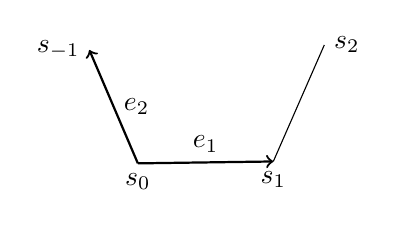
\begin{tikzpicture}[scale=.8]
\coordinate (o) at (0,0); \coordinate (a) at (2.15,.03); \coordinate (b) at (-.77,1.8); \coordinate (c) at (2.96,1.88);
\draw[->,thick] (o)--node[above] {$e_1$} (a); \draw[->,thick] (o)--node[right] {$e_2$} (b); \draw (a)--(c);
\node[below] at (o) {$s_0$}; \node[below] at (a) {$s_1$}; \node[left] at (b) {$s_{-1}$}; \node[right] at (c) {$s_2$};
\end{tikzpicture}}

\margin{[\,\uline{NB} on s'attend à $\left\{\begin{aligned}\beta&=0\ \text{i.e. }s_2-s_{\unsure{-1|+1}}\parallel e_1\\ \alpha&=\zeta+\zeta^{-1}=2\cos\theta\end{aligned}\right.$\,]}
% archive sheet number: 81
\scanpage{83}
\uline{Ex} Repr. régulière définie par $\zeta\in k$ $(\zeta\ne\pm1)$
\[ s_i=(\zeta^i,\zeta^{-i}), \]
on trouve donc
\[ s_2-s_{-1}=(\zeta^{\unsure{1|2}},\zeta^{-2})-(\zeta^{-1},\zeta)=(\zeta^{1}-\zeta^{-1},\zeta^{-2}-\zeta) \]
parallèle à
\[ \unsure{\vert(|\parallel}s_1-s_0=(\zeta-1,\zeta^{-1}-1) \]
de façon précise on a
\[ \left\{\begin{aligned}(s_2-s_{-1})&=(1+\zeta+\zeta^{-1})(s_1-s_0)=(1+\alpha)(s_1-s_0)\\
&\text{avec}\qquad \alpha=\zeta+\zeta^{-1}\end{aligned}\right. \tag*{(\unsure{xx|17})} \]
\deleted{\unsure{puisque}} \deleted{\unsure{6|\(\beta\)}}\unsure{3}

On a donc envie d'imposer la condition
\[ \beta=0. \]

\uline{Proposition} Conditions équivalentes

\[ (\mathrm i)\quad \beta=0 \]
\[ \left\{\begin{aligned}(\mathrm{ii})\quad &s_2-s_{-1}\deleted{\unsure{+\beta|\parallel}}=(1+\alpha)(s_1-s_0)\\
(\mathrm{ii}')\quad &s_2-s_{-1}\parallel s_1-s_0\\
(\mathrm{iii})\quad &\forall n\in\mathbb Z\quad s_{n+3}-s_n\unsure{\vert|\parallel}=(1+\alpha)(s_{n+2}-s_{n+1})\\
(\mathrm{iii}')\quad &\forall n\in\mathbb Z\quad s_{n+3}-s_n=(1+\alpha)(s_{n+2}-s_{n+1})\end{aligned}\right. \]
\[ \left\{\begin{aligned}(\mathrm{iv})\quad &\deleted{\unsure{\Leftrightarrow}}\det\sigma_{0V}=-1\\
(\mathrm{iv}')\quad &\det u_V=1\\
(\mathrm{iv}'')\quad &\operatorname{Tr}\sigma_{0V}=0\end{aligned}\right. \]
\deleted{(v) $\sigma_{0V}$ est une \uline{réflexion}, i.e. est $\ne\unsure{i|\mathrm{id}}$}
% archive sheet number: 82
\scanpage{84}
i.e. on a
\[ \sigma_0=\begin{pmatrix}-1&\deleted{\unsure{1+}}\alpha&1\\0&\deleted{\unsure{2}}1+\beta&0\\0&0&1\end{pmatrix} \tag*{(17)} \]
\[ \sigma_0(x,y)=(1-x+\deleted{\unsure{(1+}}\alpha y,(1+\beta)y) \tag*{(18)} \]
\[ \left\{\begin{aligned}&\left\{\begin{aligned}\sigma_1s_0&=s_0\\
\sigma_1s_1&=s_{-1}\\
\sigma_1s_{-1}&=s_1\end{aligned}\right.\\
&\left\{\begin{aligned}\sigma_1e_1&=e_2\\
\sigma_1e_2&=e_1\end{aligned}\right.\end{aligned}\right.\qquad\text{i.e.} \tag*{(\deleted{\unsure{18}}19)} \]
\[ \sigma_1=\begin{pmatrix}0&1&0\\1&0&0\\0&0&1\end{pmatrix} \tag*{(20)} \]
\[ \sigma_1(x,y)\unsure{{:}|{=}}(y,x) \tag*{(21)} \]

Il reste à écrire la condition $\sigma_0^2=\operatorname{id}$.
On trouve
\[ \left\{\begin{aligned}&\boxed{\alpha\beta=0}\qquad\deleted{(1+\beta)^2=1}\\
&(1+\beta)^2=1\quad\text{i.e}\quad\boxed{\beta^2+2\beta=0}\quad\text{i.e}\quad\boxed{\beta(\beta+2)=0}\end{aligned}\right. \tag*{\deleted{\unsure{(22)}}} \]
Donc :

\begin{tabular}{|p{.91\linewidth}}\uline{Proposition} Les représentations géom affines
régulières de $\Pi_\infty$ \inserted{sur $k$} sont \deleted{définies} en corr.
1-1 \unsure{can.|corr.} avec les couples $(\alpha,\beta)$ d'éléments
de $k$ satisfaisant les conditions
\[ \alpha\beta=(\beta+2)\beta=0 \tag*{(22)} \]
\end{tabular}
% archive sheet number: 83
\scanpage{85}
(v) On n'est pas dans le ``cas \deleted{\unsure{aberrant}} \inserted{impropre}'' suivant \inserted{$(\alpha=0,\beta=-2)$}
\[ \left\{\begin{aligned}&\deleted{\unsure{p\ne2}}\ \operatorname{car} k=p\ne2,\quad \sigma_0=\begin{pmatrix}-1&0&1\\0&-1&0\\0&0&1\end{pmatrix}\quad\text{i.e }\deleted{\sigma_0\text{ est}}\\
&\deleted{\text{la symétr}\unsure{\text{ie}}}\\
&\sigma_0(x,y)=(1-x,-y)\quad\text{i.e }\sigma_0=\text{symétrie p.r. au}\\
&\text{milieu du segment }(s_0,s_1)\end{aligned}\right. \tag*{(23)} \]

\uline{Dém} L'équivalence de (i), (ii), (ii') résulte
$\text{trivial}^{t}.$ de
\[ s_2-s_{-1}=\deleted{\unsure{\beta}}(1+\alpha)e_1+\beta e_2 \]
et du fait que $e_1=s_1-s_0$ et $e_2$ font une
base de $V$. L'équivalence de (ii) et (iii),
ou (ii') et (iii'), s'obtient en \deleted{\unsure{faisan|faisant}} notant
que pour $n=-1$ on obtient les conditions de
(ii) (iii), et qu'inversement (ii') (iii') s'obtiennent
de (ii) (iii) en appliquant $u^{n+1}$. On a
\[ \deleted{\unsure{\det\sigma_{0V}=}}\left\{\begin{aligned}\det u_V&=-\det\sigma_{0V}=1+\beta\\
\operatorname{Tr}\sigma_{0V}&=\beta\end{aligned}\right. \tag*{(24)} \]
ce qui prouve l'équivalence de (iv) \unsure{:|.} (iv') (iv'')
avec les autres conditions. Enfin, l'équivalence
avec (v) est évidente par la \deleted{\unsure{proposition|propos}}
formule (22).

\uline{Remarques sur le cas impropre} À isom unique
près, il y en a un et un seul pour \unsure{tt} $k$
% archive sheet number: 84
\scanpage{86}
donné. On a dans ce cas
\[ \left\{\begin{aligned}u(x,y)&=(1-y,-x)\\
u(x,y)&=(x+1,y-1)\end{aligned}\right. \tag*{(25)} \]
i.e. $u^2$ est la translation par le vecteur $(1,-1)$.
Donc en car. $0$ $u^2$ est d'ordre infini, donc
a fortiori $u$ l'est, donc la réalisation obtenue
de $\Pi_\infty$ est d'ordre infini (on trouve
qu'elle est fidèle\ldots) En car. $p>0$, $u^2$ est
d'ordre $p$, donc $u$ d'ordre $2p$, on trouve
\deleted{\unsure{un $2p$|un $2p$-}} donc que la réalisation géom impropre
se factorise par $\Pi_{2p}$. On vérifie
aisément que la réalisation géom de $\Pi_{2p}$
est bel et bien fidèle, donc donne un
$2p$-polygône régulier.

Avec la théorie projective des polygônes
réguliers, l'anomalie \unsure{apparente} des ``polygônes
réguliers impropres'' s'explique complètement, et on voit que du point de vue
projectif on n'a rien perdu en excluant
le cas impropre, ce qu'on fera désormais.

\uline{Scholie} Le cas d'une réalisation géom
\margin{terminologie ``invariant numérique''}
régulière \uline{propre} de $\Pi_\infty$ est classé par $\alpha\in k$,
qu'on peut choisir arbitrairement\ldots
% archive sheet number: 85
\scanpage{87}
3. \uline{Points fixes de} $\sigma_0,\sigma_1$, \uline{centre} de \uline{la réal. géom.}

\[ \left\{\begin{aligned}\sigma_0(x,y)&=(1-x+\alpha y,y)\\
\sigma_1(x,y)&=(y,x)\\
u(x,y)&=\sigma_0\sigma_1(x,y)=(1-y+\alpha x,x)\end{aligned}\right. \tag*{(26)} \]

\figure{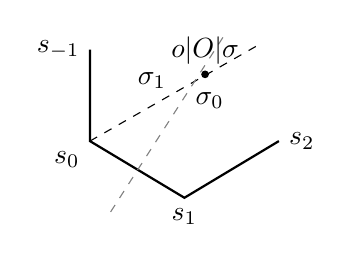
\begin{tikzpicture}[x=.75cm,y=.75cm]
\draw[thick] (0,1.55) node[left] {$s_{-1}$} -- (0,0) node[below left] {$s_0$} -- (1.6,-.96) node[below] {$s_1$} -- (3.2,0) node[right] {$s_2$};
\draw[dashed] (0,0) -- (2.84,1.62);
\draw[thin,gray,dashed] (.35,-1.2) -- (2.30,1.83);
\fill (1.95,1.13) circle (1.4pt) node[above] {$\unsure{o|O|\sigma}$};
\node at (1.05,1.02) {$\sigma_1$}; \node at (2.03,.69) {$\sigma_0$};
\end{tikzpicture}}

Points fixes de $\sigma_0$ :
\[ H_0:\quad 2x-\alpha y-1=0 \tag*{(27)} \]
c'est une droite,
sauf pour $p=2,\alpha=2$
(cas du carré en car. $2$)
où on trouve $H_0=\varnothing$. Mais
\inserted{passant} en coordonnées hom, on
trouve encore une droite
$z=0$ : la droite à l'infini
(Dans ce cas, $\sigma_0$ est la translation par $\deleted{\unsure{e}} e_1$)

Points fixes de $\sigma_1$
\[ H_1:\quad x-y=0 \tag*{(28)} \]
c'est une droite

\uline{NB} Un automorphisme affine \inserted{d'un plan affine} \unsure{dont|que} l'ens des
points fixes est une droite est appelé une
\uline{réflexion affine}. On voit donc que le
cas ``propre'' de la proposition précédente est
caractérisé aussi par la condition

(iv''') $\sigma_0$ est une réflexion affine, ou \deleted{\unsure{à|a}} une
translation \deleted{(dans le} \inserted{(ce dernier cas \deleted{\unsure{seulmt}}} dans le seul cas
$p=2,\alpha=0$ i.e. carré en car. $2$, et alors $\sigma_0$ est
encore une réflexion projective\ldots)
% archive sheet number: 86
\scanpage{88}
$(\mathrm{iv}^{(\mathrm{iv})})$ $\sigma_{0V}$ est une réflexion, ou l'identité
(avec \deleted{\unsure{la|sa}} remarque)

\uline{NB} Dans le cas impropre, $\sigma_{0\unsure{E|k}}$ est la sym. p.r. à
un pt (car. $\ne2$), $\sigma_{0V}$ est la symétrie $\deleted{\unsure{v}}v\mapsto-v$.

\uline{Points fixes sous} $G$ = \uline{pts fixes sous} $G^+$ = \uline{pts}
\uline{fixes sous} $u$ :
% slanted
\margin{\uline{terminologie} \uline{Centre} de la réalisation géom de $\Pi_\infty$\ldots}
\[ x_0=y_0=\frac{1}{2-\alpha} \tag*{(29)} \]
(qui existe ssi $\alpha\ne2$, et est tjrs unique)

4. \uline{Valeurs propres de} $u_V$. \uline{Comparaison avec}
\uline{les} $\unsure{\varphi\zeta|\varphi_\zeta}$\ldots

\[ u_V=\begin{pmatrix}\alpha&-1\\1&0\end{pmatrix} \tag*{(30)} \]
\[ \deleted{\unsure{\det(|\det}} \left\{\begin{aligned}\det u_V&=1\\
\operatorname{Tr} u_V&=\alpha\end{aligned}\right. \tag*{(31)} \]
\unsure{équations|équation} aux valeurs propres $(\zeta,\in\overline{k})$
\[ \unsure{\zeta^2|\zeta}-\alpha\zeta+1=0\qquad\text{discriminant} \tag*{(32)} \]
\[ \Delta\unsure{(\alpha)|{}}=\alpha^2-4=(\alpha-2)(\alpha+2) \tag*{(33)} \]
En termes du choix d'\uline{un} tel $\zeta$, on
trouve
\[ \alpha=\zeta+\zeta^{-1} \tag*{(33)} \]
( \uline{NB} les deux racines $\zeta,\zeta'$ de \unsure{notre|cette} équation
satisfont
\[ \left\{\begin{aligned}\zeta+\zeta'&=\alpha\\
\zeta\zeta'&=1\end{aligned}\right.\qquad\text{i.e. }\zeta'=\zeta^{-1}. \tag*{(34)} \]
% archive sheet number: 87
